%課題研究レジュメテンプレート ver. 1.2

\documentclass[uplatex]{jsarticle}
\usepackage[top=20mm,bottom=20mm,left=20mm,right=20mm]{geometry}
\usepackage[T1]{fontenc}
\usepackage{txfonts}
\usepackage{wrapfig}
\usepackage[expert,deluxe]{otf}
\usepackage[dvipdfmx,hiresbb]{graphicx}
\usepackage[dvipdfmx]{hyperref}
\usepackage{pxjahyper}
\usepackage{secdot}

\makeatletter
  \renewcommand{\section}{%
    \if@slide\clearpage\fi
    \@startsection{section}{1}{\z@}%
    {\Cvs \@plus.5\Cdp \@minus.2\Cdp}% 前アキ
    {.5\Cvs \@plus.3\Cdp}% 後アキ
    %{\normalfont\Large\headfont\raggedright}}
    {\normalfont\raggedright}}

  \renewcommand{\subsection}{\@startsection{subsection}{2}{\z@}%
    {\Cvs \@plus.5\Cdp \@minus.2\Cdp}% 前アキ
    {.5\Cvs \@plus.3\Cdp}% 後アキ
    %{\normalfont\large\headfont}}
    {\normalfont}}

  \renewcommand{\subsubsection}{\@startsection{subsubsection}{3}{\z@}%
    {\Cvs \@plus.5\Cdp \@minus.2\Cdp}%
    {\z@}%
    %{\normalfont\normalsize\headfont}}
    {\normalfont}}
\makeatother
%ここから上を編集する必要はない.

\title{\vspace{-14mm}高齢者入居施設における利用者管理システムの導入}
\author{PMコース 矢吹研究室 1442068 鈴木博文}
\date{}%日付を入れる必要はない.
\pagestyle{empty}%ページ番号は振らない.
\begin{document}
\maketitle

\section{研究の背景}

現在の日本では,少子高齢化が大きな課題の一つとなっている.日本の総人口は,2048年には1億人を割り,2060年には8,000万人になるものと見込まれている.この人口減少と反比例して,高齢人口は2010年の2,900万人から団塊の世代,及び第二次ベビーブーム世代が高齢人口に入ったあとの2042年に3,800万人とピークを迎えるものとされている.そのため,高齢化率は2013年には25.1\%で4人に1人を上回り,50年後の2060年には39.9\%すなわち2.5人に1人が65歳以上になることが見込まれている.このことから日本は,人口減少と少子高齢化の急速な進行が現実のものとなることが予測されている\cite{site1}.

高齢化率が上昇するとともに,特別養護老人ホームなどの介護が必要な高齢者が入居する施設が不足しているという点も課題の一つとされている.現在の特別養護老人ホームの入居待ちは,全国で50万人を超えるとされており,行き場のない高齢者は制度外の施設に流れるなど,一般的な老人ホームも全国で不足している\cite{site2}.

現状あるホーム内においても,満足な経営状況で運営されているとは限らない.介護職員不足に悩まされている施設も多くある.介護職員が必要な人数に対し,実際に働くことのできる人数は何人かという充足率の統計を見ると,2017年度には94\%となり,早くも6\%の介護者が不足するという推計がでている.この数字は2025年には85.1\%まで低下すると推計されているのだ\cite{site3}.

\section{研究の目的}
私は,介護者不足と高齢者入居施設不足の問題を並行して解決するためには,少ない人数で現状の作業を効率よく行なうことが必要だと考え,高齢者入居施設にWebアプリケーションを用いた利用者の管理ツールを導入すること提案する.現状で介護ソフトが導入されている例はあるが,使いづらいなどの理由から全ての機能を使いこなすことが出来ず,ソフトと紙媒体の並行使用を行なうことで余計に手間がかかっている.実際の介護施設での調査を基に新たな利用者管理のシステム開発を行い,IT技術の面から福祉を変えるきっかけとなるのを目指す.今回は実際の高齢者入居施設で記録の方法や問題点,実際にシステム化する場合に便利なる点や留意点などを調査し,調査施設独自の専用のシステムを開発する.

多くの施設では入居者に関する日常の記録は手書きで残しており,過去のデータを含めると非常に多くの紙媒体が保管されている.さらに,日中に記録されたデータは夜間に集計されることではじめて入居者一人ひとりの一日のデータとなるなど非常に多くの作業を要する.これをWebアプリケーションに置き換えることでスマートフォンやタブレット端末,コンピュータなど様々な端末からアクセスができ,同時に双方向から記録することが可能となる.作業量を軽減するために,集計などを自動化するほか,ヒューマンエラーによる入力漏れや誤入力を防止するため,異常数値を検出した場合に利用者に知らせる機能を実装する.

今回はデザイン科学科の学生との共同作業とする.協力施設での調査を基にシステム化すべき項目を共同で決定し,デザイン科の学生がデザイン案を制作する.デザイン案をもとに自身がWebアプリケーションを構築する.

\section{プロジェクトマネジメントとの関連}

当研究はPMBOKにおいてプロジェクト・スコープ・マネジメントと関連すると考える.プロダクトを作るにあたって,ステークホルダが必要とする成果物を納品するために,ツールと技法にインタビューを用いるためである.ステークホルダが必要としている機能や要求はインタビューを行なうことで明らかにされる.今回のプロダクトは,調査する施設独自の専用のシステムを開発することから,ステークホルダが本当に必要とする機能や要求を直接聞くことが重要である.

\section{研究の方法}

\begin{wrapfigure}[6]{r}{7cm}
\vspace*{-\intextsep}
%\includegraphics[width=図の幅,clip]{ファイル名}\label{参照用ラベル}
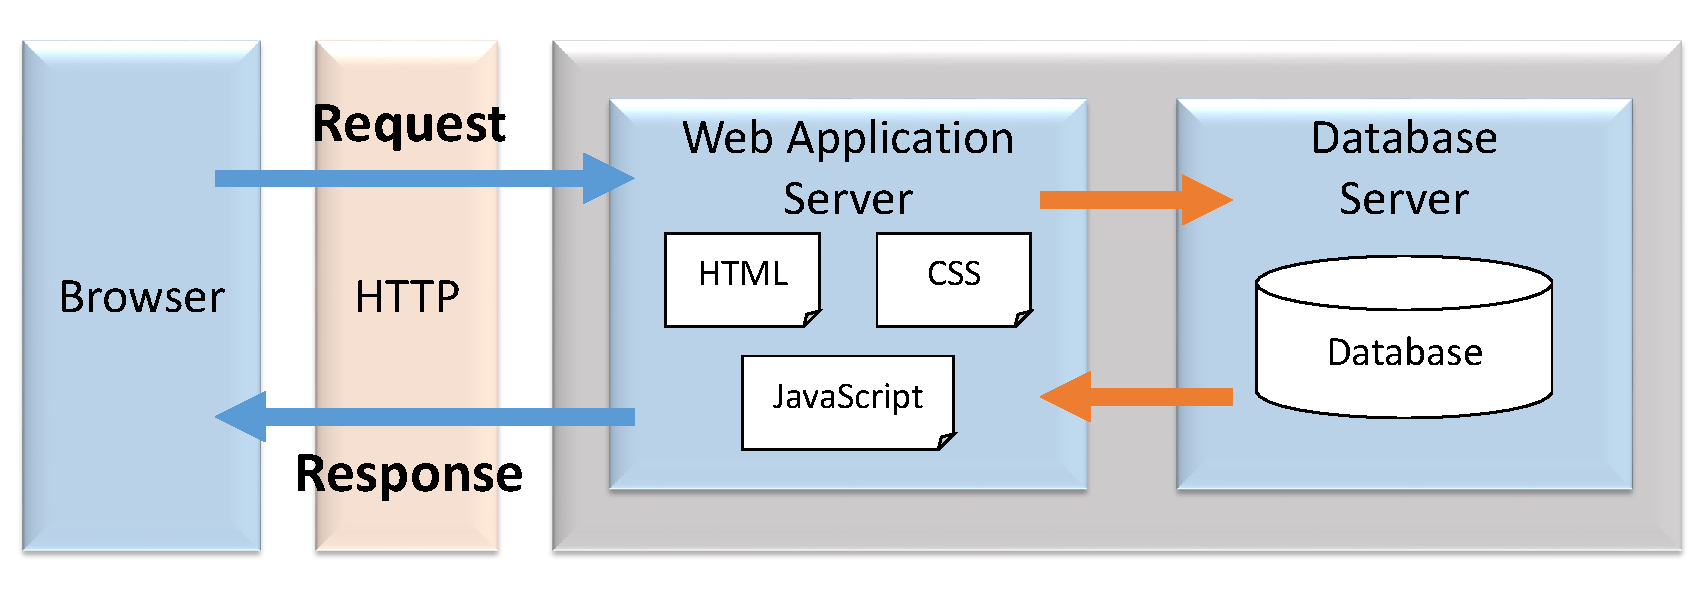
\includegraphics[width=8cm,clip]{figure.pdf}
\caption{アーキテクチャ図}\label{アーキテクチャ}
\end{wrapfigure}

\subsection{システムの構築環境}

当システムはブラウザを通しアクセスする.CSSを用いて,シンプルで操作しやすい画面デザインを設計する.さらに,JavaScriptを使用した動的な画面遷移も取り入れる.利用者情報の入出力は,データベースサーバー上のデータベースに接続し,記録・抽出する.情報の抽出は,現場で必要とされている項目を中心に検索するよう設計し,利用者に対しレスポンスする.本システムのアーキテクチャを図\ref{アーキテクチャ}に示す.

\subsection{ハイレベルな要求事項}
本研究内にて重要とされる実現項目は次の通りである.
\begin{enumerate}
\item 入力値の異常を使用者に的確に知らせ,入力漏れや誤入力を防止する.
\item 機器操作を不慣れとする人にも操作しやすい画面設計とする.
\item 実際の現場で使用するにあたり,使用頻度の高い項目を重点的にシステム化する.
\end{enumerate}

\subsection{プロダクトの評価}

当システムは実際の高齢者入居施設に勤務する介護スタッフ・看護師記録を担当とする方々に実際に使用してもらう.ソフトの基本動作の説明を行い,実際に操作を行ってもらう.その様子を観察するとともに操作後に使用の感想や改善点を再度インタビューし,調査対象の施設で使用するにあたって,より独自性の高いシステムを開発する.

\section{現在の進捗状況}

協力施設にシステム化すべき項目を聞き,システムを開発した.16年11月中旬に開発したシステムを協力施設にて担当者に説明を行い一部運用,改善すべき点と評価点をインタビューした.現地での調査によって,優先的にシステム化してほしいことについての情報を得ることができ,効率よく記録を行うための作業の流れについて聞くことができた.その後改善点を中心にシステムを変更.新規で追加すべき項目を洗い出しシステム開発を継続中である.

\section{今後の計画}
以下の手順で研究を進める予定である.
\begin{enumerate}
\item 1月中旬を目処にシステム全体の推移とデータ管理を完成させる.
\item 2月上旬にシステムを完成させる.
\end{enumerate}
\bibliographystyle{junsrt}
\bibliography{biblio}%「biblio.bib」というファイルが必要.

\end{document}
